\documentclass[a4paper,12pt]{article}

\usepackage[T2A]{fontenc}			
\usepackage[utf8]{inputenc}			
\usepackage[english,russian]{babel}	

\usepackage[
bookmarks=true, colorlinks=true, unicode=true,
urlcolor=black,linkcolor=black, anchorcolor=black,
citecolor=black, menucolor=black, filecolor=black,
]{hyperref}

\usepackage{color}
\usepackage{caption}
\DeclareCaptionFont{white}{\color{black}}
\DeclareCaptionFormat{listing}{\colorbox{white}{\parbox{\textwidth}{#1#2#3}}}
\captionsetup[lstlisting]{format=listing,labelfont=white,textfont=white}

\usepackage{amsmath,amsfonts,amssymb,amsthm,mathtools} 
\usepackage{wasysym}

\usepackage{graphicx}
%\usepackage[cache=false]{minted}
\usepackage{cmap}
\usepackage{indentfirst}

\usepackage{listings}

\usepackage{fancyvrb}

\usepackage{geometry}
\geometry{left=2cm}
\geometry{right=1.5cm}
\geometry{top=1cm}
\geometry{bottom=2cm}

\setlength{\parindent}{5ex}
\setlength{\parskip}{0.5em}

\usepackage{pgfplots}
\usetikzlibrary{datavisualization}
\usetikzlibrary{datavisualization.formats.functions}

\begin{document}
	\lstset{ %
		language=C,                 % выбор языка для подсветки (здесь это С)
		basicstyle=\small\sffamily, % размер и начертание шрифта для подсветки кода
		numbers=left,               % где поставить нумерацию строк (слева\справа)
		numberstyle=\tiny,           % размер шрифта для номеров строк
		stepnumber=1,                   % размер шага между двумя номерами строк
		numbersep=5pt,                % как далеко отстоят номера строк от подсвечиваемого кода
		backgroundcolor=\color{white}, % цвет фона подсветки - используем \usepackage{color}
		showspaces=false,            % показывать или нет пробелы специальными отступами
		showstringspaces=false,      % показывать или нет пробелы в строках
		showtabs=false,             % показывать или нет табуляцию в строках
		frame=single,              % рисовать рамку вокруг кода
		tabsize=2,                 % размер табуляции по умолчанию равен 2 пробелам
		captionpos=t,              % позиция заголовка вверху [t] или внизу [b] 
		breaklines=true,           % автоматически переносить строки (да\нет)
		breakatwhitespace=false, % переносить строки только если есть пробел
		escapeinside={\%*}{*)}   % если нужно добавить комментарии в коде
	}
	
	% Титульный лист
	\begin{figure}[h!]
		\begin{center}
			{
\includegraphics[scale = 0.8]{titul.pdf}}
			\label{titul}
		\end{center}
	\end{figure}

	\pagestyle{empty} %  выключаенм нумерацию
	
	\newpage
	
	\section*{Индивидуальное задание}
	
	Проанализировать существующие системы автоматического анализа обзоров, использующих механизмы AI  и обработки больших данных. На указанном примере автоматизировать выгрузку ревью, идентифицировать ключевые категории оценки продукта пользователями (стабильность, энергопотребление, конкретная функциональность и т.д.), реализовать автоматизированный подсчет количества положительных и отрицательных отзывов по конкретным категориям, автоматизировать оценку трендов изменения оценки категорий по годам, кварталам или месяцам.
	
	\newpage
	
	\tableofcontents
	
	\newpage
	
	\section*{Введение}
	\addcontentsline{toc}{section}{Введение}
	
	На сегодняшний день магазины приложений, такие как Google Play или Apple Store, различные Web-сайты позволяют пользователям оставлять отзывы об используемых сервисах, публикуя комментарии и выставляя оценки. Эти платформы представляют собой полезный электронный ресурс,
	в котором разработчики приложений и пользователи могут продуктивно обмениваться информацией о сервисах. 
	
	В частности, отзывы пользователей могут содержать опыт использования приложений, сообщения об ошибках и предложения для улучшения сервиса. Вся эта информация может помочь разработчикам приложений выполнять задачи по сопровождению, развитию и модификации программного обеспечения. Однако большой объем полученных отзывов, их неструктурированный характер и различное качество могут сделать выявление полезных отзывов пользователей очень сложной задачей, на которую придется тратить много времени.
	
	Таким образом, возникает потребность в автоматизации этого процесса, используя механизмы AI и обработки больших данных.
	
	\textbf{Цель практики:} проанализировать существующие системы автоматического анализа обзоров, использующих механизмы AI и обработки больших данных, и применить полученные знания на практике.
	
	\textbf{Задачи работы:}
	
	\begin{enumerate}
		\item изучить существующие подходы автоматического анализа обзоров, использующих механизмы AI и обработки больших данных;
		\item выбрать наиболее подходящие из них для решения индивидуального задания;
		\item автоматизировать выгрузку ревью продукта Parallels Desktop;
		\item идентифицировать ключевые категории оценки продукта пользователями;
		\item реализовать автоматизированный подсчет количества положительных и отрицательных отзывов по конкретным категориям;
		\item автоматизировать оценку трендов изменения оценки категорий по годам, кварталам или месяцам.
	\end{enumerate}

	\pagestyle{plain} % включаем нумерацию
	\pagebreak
	
	\section{Аналитический раздел}
	
	В данном разделе будут описаны существующие подходы автоматического анализа обзоров, использующих механизмы AI и обработки больших данных; идентификация ключевых категорий оценки продукта пользователями; подготовка данных для обучения модели и метод, использующийся для ее обучения.
	
	Оценка трендов изменения оценки категорий по годам, кварталам или месяцам в данной работе не производилась, поскольку данный материал слишком обширный, и на его изучение требуется больше времени, чем отводится в рамках учебной практики.
	
	\subsection{Подходы автоматического анализа обзоров, использующих механизмы AI и обработки больших данных}
	
	Процесс анализа, классификации и выбора отзывов пользователей, полезных для разработчиков, состоит из 4 шагов~\cite{university}:
	
	\begin{itemize}
		\item Таксономия обслуживания и развития программного обеспечения (Taxonomy for Software Maintenance and Evolution).
		
		Она подразумевает анализ отзывов конкретного программного обеспечения и выделения ключевых категорий, наиболее полезных для разработчиков.
		
		\item Извлечение признаков (Feature Extraction).
		
		Целью данного шага является извлечение набора наиболее значащих признаков из отзывов пользователей, которые потом будут использованы алгоритмами машинного обучения.
		
		\item Обучение модели на основе выделенных признаков (Learning Classifiers).
		
		\item Оценка полученных результатов (Evaluation).
	\end{itemize}

	Рассмотрим поподробнее каждый из них.
	
	\subsection{Идентификация ключевых категорий оценки продукта пользователями (Taxonomy)}
	
	Цель этого первого шага состоит в том, чтобы вывести таксономию категорий отзывов пользователей, которая имеет отношение к обслуживанию и развитию программного обеспечения.
	
	Чтобы достичь поставленной цели необходимо проанализировать отзывы пользователей и ответы разработчиков на них. Анализ выполняется вручную.
	
	\subsection{Подготовка данных для обучения модели (Feature Extraction)}
	
	Существуют три основных этапа, применяющихся для анализа содержания отзывов приложений и извлечения наиболее важных признаков (features) для следующего шага (Learning Classifiers):
	
	\begin{itemize}
		\item Text Analysis (TA);
		
		Этот этап включает в себя выбор метода, подходящего для извлечения наиболее важной информации из текста (textual features). Он состоит из двух этапов:
		
		\begin{itemize}
			\item Предварительная обработка текста (Preprocessing).
			
			Все слова, содержащиеся в нашем наборе отзывов пользователей, используются в качестве информационной базы для создания текстового вокабуляра, который подвергается предварительной обработке с применением удаления стоп-слов (предлогов, союзов, знаков и тд) и lemmatization (преобразует слова в начальную форму).
			
			\item Векторизация текста (Textual Feature Weighting).
			
			Существует множество способов векторизовать текст, но наиболее популярные, зарекомендовавшие себя, способы - это TF-IDF, прямое и частотное кодирование. В данной работе используется частотное кодирование, суть которого заключается в том, чтобы представить каждый отзыв в виде вектора, элементы которого являются числом вхождения каждого слова из вокабуляра, полученного на предыдущем этапе.
		\end{itemize}
		\item Natural Language Processing (NLP);
		
		Этот этап включает в себя в нахождении рекуррентных лингвистических шаблонов среди отзывов, которые можно будет использовать для распознавания предложений, относящихся к той или иной категории (Раздел 1.2 Taxonomy).
		
		Поскольку задача подразумевает просмотр и глубокий ручной анализ большого количества отзывов для нахождения подобных шаблонов (рис. ), а времени на ее реализацию не достаточно в рамках учебной практики, было решено классифицировать все отзывы вручную, не прибегая к поиску шаблонов.
		
		\item Sentiment Analysis (SA).
		
		Анализ настроений - это процесс присвоения количественного значения фрагменту текста, выражающему аффект или настроение. В данной работе рассматривается анализ настроений как задача классификации текста, которая присваивает каждый отзыв одному соответствующему классу. 
		
		Для решения этой задачи классы определяются как три различных уровня интенсивности настроения: положительный, отрицательный и нейтральный. 
		
		В качестве модели для прогнозирования настроений отзывов пользователей было решено использовать модель дискретного Наивного Байесовоского классификатора, поскольку в источнике ~\cite{university} говорится, что наивный байесовский метод показывает лучшие результаты, чем другие алгоритмы машинного обучения, традиционно используемые для классификации текста при анализе настроений.
	\end{itemize}
	
	
	
	\subsection*{Выводы}
	\addcontentsline{toc}{subsection}{Выводы}
	
	\begin{itemize}
		\item Были изучены подходы, использующиеся для автоматического анализа отзывов, использующих механизмы AI и обработки больших данных; и выделены их основные этапы: Taxonomy, Feature Extraction, Learning Classifiers, Evaluation.
		
		\item Было решено выполнять таксономию вручную.
		
		\item Были выделены и подробно разобраны основные этапы извлечения признаков (Feature Extraction). Для каждого этапа был выбран метод, позволяющий решить поставленную задачу.
		
		\item Также, было решено не выполнять оценку трендов изменения оценки категорий по годам, кварталам или месяцам вследствие нехватки времени на поставленную задачу.
	\end{itemize}
	
	\section{Конструкторский раздел}
	
	В этом разделе приводится описание сбора данных (отзывов), предварительной обработки и векторизации, а также особенности обучения и тестирования модели на собранных данных.
	
	\subsection{Сбор данных}
	
	Отзывы были предоставлены ментором данного задания из источника~\cite{parallels} - всего 284 шт.
	
	Очевидно, что такого количества недостаточно, чтобы обучить и протестировать модель, поэтому было принято решение добавить отзывы из магазина приложений App Store~\cite{appstore} с помощью ресурса Appfigures~\cite{appfigures}, предоставляющего API к App Store.
	
	Поскольку большинство отзывов написано на английском языке, оставшиеся отзывы были переведены на английский язык. Итого получилось 1023 отзыва, что безусловно мало для полноценного обучения и тестирования модели, но достаточно, чтоб получить хоть какие-то вменяемые результаты.
	
	Каждому отзыву соответсвует оценка по пятибальной шкале: от 1-5. Если оценка меньше 3, то отзыв будет считаться отрицательным (всего 525 шт.), если больше 3 (363), то положительным, и если равно 3, то нейтральным (всего 160 шт.).
	
	Все отзывы были разбиты по соответствующим категориям:
	
	\begin{itemize}
		\item Лицензия, пробная версия, цена (390 шт.).
		
		Пример отзыва: \textit{Paid for 1 year for 3990 rubles, but the license was not activated !!! The support servant is silent, what should I do?}
		
		\item Функциональность (качество работы утилит, программ, настроек) (174 шт.).
		
		Пример отзыва: \textit{Does not have OpenGL support in the NVIDIA Geforce GT 750M drivers for Linux. So unfortunatly the whole purpose of using Linux to avoid Mac depriciating OpenGL/OpenCL for 3D rendering is undermined by the lack of support in the driver too. From what I have read this is true for Windows graphics card drivers in Parallels as well.}
		
		\item Производительность и скорость работы (50 шт.).
		
		Пример отзыва: \textit{Downloading win system is too slow, 500m broadband, 9 hours to download 5g win10, drunk}
		
		\item Установка и работа системы, интеграция (251 шт.).
		
		Пример отзыва: \textit{I used the trial version to decide if Parallels was worth the investment. I was pleasantly surprised with the ease of installation and configuration. I installed both Windows 10 and Ubuntu 18.04 on my iMac-Pro, with Catalina.  Both worked flawlessly.}
		
		\item Отзывы, не несущие полезную информацию для разработчика (158 шт.).
		
		Пример отзыва: \textit{very good}
	\end{itemize}
	
	\subsection{Предварительная обработка}
	
	Предварительная обработка включает в себя токенизацию отзывов (разбиение текста на слова и биграммы), нормализацию получившихся слов и создание текстового вокабуляра слов.
	
	Нормализация будет осуществляться посредством приведения слов к нижнему регистру, удалению стоп-слов (предлогов, союзов знаков, символов и тд) и лемматизации (приведению слов к начальной форме).
	
	Вокабуляр будет содержать в себе список наиболее часто встречающихся нормализованных слов.
	
	Итого, на выходе этого этапа получается список токенизированных и нормализованных отзывов и вокабуляр слов.
	
	\subsection{Векторизация}
	
	Как уже было сказано ранее, для векторизации текста в данной работе будет использоваться частотное кодирование.
	
	То есть каждый отзыв будет представлять из себя вектор, элементы которого являются числом вхождения каждого слова из вокабуляра.
	
	\subsection{Обучение и тестирование модели}
	
	В качестве модели используется модель Наивного Байесовского классификатора (дискретного).
	
	Байесовский классификатор имеет гиперпараметр $alpha$, который отвечает за сглаживание модели. Наивный Байес вычисляет вероятности принадлежности каждого отзыва ко всем классам, для этого перемножая условные вероятности появления всех слов отзыва, при условии принадлежности к тому или иному классу. Но если какое-то слово отзыва не встречалось в обучающем наборе данных, то его условная вероятность равна нулю, что обнуляет вероятности принадлежности отзыва к какому-либо классу. Чтобы избежать этого, по умолчанию ко всем условным вероятностям слов добавляется единица, то есть alpha равняется одному. Однако это значение может быть неоптимальным. Поэтому его значение будет определено в процессе выполнения эксперимента с помощью поиска по сетке и кросс валидации.
	
	Данные будут разбиты на две части - обучающую и тестирующую, в соотношении 3:1, соответственно.
	
	\subsection*{Выводы}
	\addcontentsline{toc}{subsection}{Выводы}
	
	В разделе были даны описания сбора данных (отзывов), предварительной обработки и векторизации, а также особенности обучения и тестирования модели на собранных данных.
	
	\newpage
	
	\section{Технологический раздел}
	
	Здесь описываются требования к программному 
	обеспечению и средства реализации, приводятся листинги 
	программы.
	
	\subsection{Требования к программному обеспечению}
	
	Необходимо подготовить программный комплекс, который будет считывать отзывы из файла формата csv, преобразовывать их в список и далее обрабатывать в соответствии со схемой изложенной в Конструкторском разделе.
	
	На выходе получается обученная модель, готовая для тестирования.
	
	\subsection{Средства реализации}
	
	Для реализации поставленной задачи был использован язык программирования Python~\cite{python}. Проект был выполнен в среде The Jupyter Notebook~\cite{notebook}.
	
	Используемые библиотеки: nltk~\cite{nltk}, scipy и numpy~\cite{scipy_numpy}, pandas~\cite{pandas}.
	
	\subsection{Листинг программы}
	
	Реализованный программный комплекс представлен
	в листингах \ref{lst0}-\ref{lst2}.
	
	\begin{lstlisting}[label=lst0,caption=Предварительная обработка]
	import nltk
	from nltk.corpus import PlaintextCorpusReader
	from nltk.probability  import FreqDist
	from nltk.tokenize import RegexpTokenizer
	from nltk import bigrams
	from nltk import pos_tag
	from nltk.stem import WordNetLemmatizer
	from collections import OrderedDict
	from sklearn.metrics import classification_report, accuracy_score
	from sklearn.naive_bayes import MultinomialNB
	from sklearn.model_selection import GridSearchCV
	from sklearn.utils import shuffle
	from multiprocessing import Pool
	import numpy as np
	from scipy.sparse import csr_matrix
	import pandas as pd
	
	def lower_pos_tag(words):
		lower_words = []
		for i in words:
			lower_words.append(i.lower())
		pos_words = pos_tag(lower_words)
		return pos_words
		
	def clean(words):
		wordnet_lemmatizer = WordNetLemmatizer()
		cleaned_words = []
		types = ['JJ', 'JJR', 'JJS', 
					'MD', 'NN', 'NNS', 
					'NP', 'NPS', 'POS', 
					'PP', 'RB', 'RBR', 
					'RBS', 'VV', 'VVD', 
					'VVG', 'VVN', 'VVP', 'VVZ']
		for i in words:
			if i[1] in types:
			cleaned_words.append(wordnet_lemmatizer.lemmatize(i[0]))
		return cleaned_words
		
	def get_review_by_status(data_path, status):
		frame = pd.read_csv(data_path, header=0, sep=',')
		return frame[frame['status'].isin([status])].review.to_list()
		
	def get_review_by_label(data_path, label):
		if (label == 'neutral'):
			return get_review_by_status(data_path, 0)
		elif (label == 'bad'):
			return get_review_by_status(data_path, -1)
		elif (label == 'good'):
			return get_review_by_status(data_path, 1)
		else:
			return None
	
	def process(data_path, label):
		# Wordmatrix - list of reviews with tokens
		# All words - list of all words
		data = {'Word_matrix': [], 'All_words': []}
		# Intermediate list for removing gapaxes
		templist_allwords = []
		reviews = get_review_by_label(data_path, label)
		# Creating a tokenizer
		tokenizer = RegexpTokenizer(r'\w+|[^\w\s]+')
		for review in reviews: # Case processing
			bag_words = tokenizer.tokenize(review)
			lower_words = lower_pos_tag(bag_words)
			cleaned_words = clean(lower_words)
			finalist = list(bigrams(cleaned_words)) + cleaned_words
			data['Word_matrix'].append(finalist)
			templist_allwords.extend(cleaned_words)
		# Definition of hapaxes
		templistfreq = FreqDist(templist_allwords)
		hapaxes = templistfreq.hapaxes()
		# Filtration from gapaxes
		for word in templist_allwords:
			if word not in hapaxes:
			data['All_words'].append(word)
		return {label: data}
	\end{lstlisting}
	
	\begin{lstlisting}[label=lst1,caption=Векторизация]
	# Create tagged data with structure:
	# [([list of review words], class_label)]
	def union_data(data):
		labels = ['neutral', 'bad', 'good']
		labeled_data = []
		for label in labels:
			for document in data[label]['Word_matrix']:
			labeled_data.append((document, label))
		return labeled_data
	
	def vocabular_create(labels, data):
		# Creating a vocabulary with unique tokens
		all_words = [] 
		for label in labels:
			frequency = FreqDist(data[label]['All_words'])
			common_words = frequency.most_common(1000)
			words = [i[0] for i in common_words]
			all_words.extend(words)
		# Extraction of unique tokens
		unique_words = list(OrderedDict.fromkeys(all_words))
		return unique_words
	
	 def frequency_coding(labeled_data, unique_words):
		# Frequency coding for classifiers scikit-learn
		# Sparse matrix for features
		matrix_vec = csr_matrix((len(labeled_data), len(unique_words)), dtype=np.int8).toarray()
		# Array for class labels
		target = np.zeros(len(labeled_data), 'str')
		for index_doc, document in enumerate(labeled_data):
			for index_word, word in enumerate(unique_words):
				# Counting the number of occurrences of a word in the review
				matrix_vec[index_doc, index_word] = document[0].count(word)
			target[index_doc] = document[1]
		return matrix_vec, target
	\end{lstlisting}
	
	\begin{lstlisting}[label=lst2,caption=Обучение модели]
	# Reading, processing and vectorization of training data
	teaching_data = {}
	labels = ['neutral', 'bad', 'good']
	for label in labels:
	teaching_data.update(process('teaching_sentiments.csv', label))
	
	unique_words = vocabular_create(labels, teaching_data)
	
	matrix_vec, target = frequency_coding(union_data(teaching_data), unique_words)
	
	# Shuffling the dataset
	X, Y = shuffle(matrix_vec, target)
	
	model = MultinomialNB(0.1)
	model.fit(X, Y)
	\end{lstlisting}
	
	\subsection*{Выводы}
	\addcontentsline{toc}{subsection}{Выводы}
	
	В данном разделе были рассмотрены требования к 
	программному обеспечению, обоснован выбор средств 
	реализации, приведены листинги программы.
	
	\newpage
	
	\section{Исследовательский раздел}
	
	В этом разделе представлены результаты работы программного комплекса на тестирующих выборках.
	
	Тестовые данные обрабатывались также, как и обучающая выборка, однако для векторизации использовался вокабуляр обучающего датасета.
	
	\begin{lstlisting}[label=lst3,caption=Тестирование модели]
	predicted = model.predict(X_test)
	# Accuracy on the control dataset
	score_test = accuracy_score(Y_test, predicted)
	# Classification report
	report = classification_report(Y_test, predicted)
	\end{lstlisting}
	
	\subsection{Тестирование на отзывах Parallels}
	
	Тестирование производилось на выборке объемом 281 отзывов ($\frac{1}{4}$ датасета).
	
	На рисунке \ref{fig:parallels} представлена таблица результатов и оценка точности.
	
	\begin{figure}[h!]
		\center{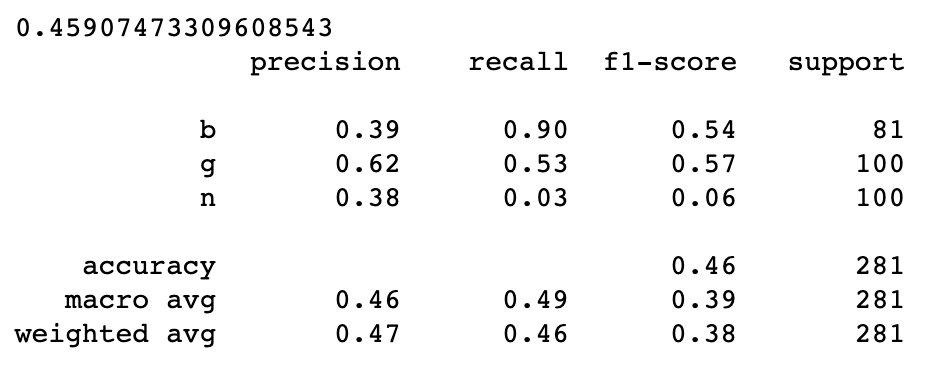
\includegraphics[width=0.5\textwidth]{parallels.png}}
		\caption{Результаты тестирования на данных Parallels}
		\label{fig:parallels}
	\end{figure}
	Где precision - доля правильно угаданных оценок (идет счет по $predicted$), recall - доля оценок, которые правильно угадали  (идет счет по $Y_test$).
	
	Видно, что точность оценки не сильно впечатляет (менее 50\%). Хоть это и лучше простого угадывания (33\%). Также, можно заметить, что модель хорошо справляется с плохими отзывами и неплохо с хорошими. Хуже всего получается предсказывать нейтральные отзывы. Можно заметить, что результаты пропорциональны количеству отзывов (плохих - 525, хороших - 363, нейтральных - 160), из чего можно сделать вывод, что модели не хватает данных, чтобы обучиться.

	
	\subsection{Тестирование на отзывах Excel}
	
	Тестирование производилось на выборке объемом 300 отзывов. Были взяты 100 положительных, 100 отрицательных и 100 нейтральных отзывов.
	
	На рисунке \ref{fig:excel} представлена таблица результатов и оценка точности.
	
	\begin{figure}[h!]
		\center{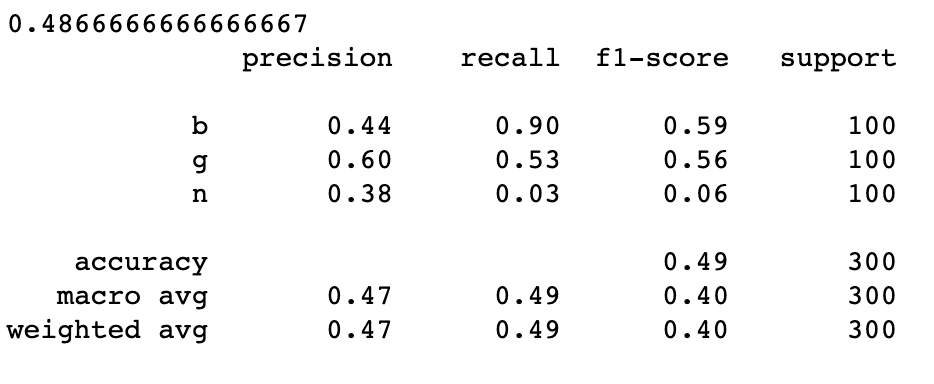
\includegraphics[width=0.5\textwidth]{excel.png}}
		\caption{Результаты тестирования на данных Excel}
		\label{fig:excel}
	\end{figure}

	Ровно такая же тенденция прослеживается на отзывах Excel, что подтверждает выводы, сделанные в предыдущем тестировании.
	
	\subsection*{Выводы}
	\addcontentsline{toc}{subsection}{Выводы}
	
	Было проведено тестирование на 2 разных группах отзывов. Оба они показывают довольно плохие плохие результаты, что связано с недостаточным количеством обучающей выборки.
	
	\newpage
	
	\section*{Заключение}
	\addcontentsline{toc}{section}{Заключение}
	
	В ходе работы выполнено следующее:
	
	\begin{enumerate} 
		\item[1)] изучены существующие подходы автоматического анализа обзоров, использующих механизмы AI и обработки больших данных;
		\item[2)] выбран наиболее подходящий из них для решения индивидуального задания;
		\item[3)] произведена выгрузка ревью продукта Parallels Desktop с сервиса Trustpilot и App Store;
		\item[4)] идентифицированы ключевые категории оценки продукта пользователями;
		\item[5)] реализован автоматический подсчет количества положительных, отрицательных и нейтральных отзывов по конкретным категориям с точностью 45,91\%;
	\end{enumerate}

	В результате проведенных тестов выяснилось, что обученная модель имеет точность предсказания 45,91\%. Такая низкая точность связана с нехваткой данных для обучения. Об этом свидетельствует прямая зависимость между распределением количества положительных, отрицательных и нейтральных отзывов в датасете и долей оценок, которые правильно угадали по соответствующему классу.
	
	Таким образом, текущую модель можно улучшить, подготовив большее количество данных (порядка 3 тыс.), примерно до 62\% точности~\cite{habr}. Это почти в два раза лучше простого угадывания, но точность все ещё довольно низка.
	
	Также, можно было бы свести задачу до бинарной классификации отзывов на положительные и отрицательные, что также повысило бы точность.
	
	
	
	\newpage
	
	\addcontentsline{toc}{section}{Список литературы}
	\begin{thebibliography}{9}
		
		\bibitem{university} How can I improve my app? Classifying user reviews for software maintenance and evolution [Электронный ресурс]. - Режим доступа: https://www.zora.uzh.ch/id/eprint/113425/1/C17.pdf, свободный. (Дата обращения: 18.07.2020 г.)
		
		\bibitem{habr} Анализ эмоциональной окраски отзывов с Кинопоиска [Электронный ресурс]. – Режим доступа: https://habr.com/ru/post/467081/, свободный. (Дата обращения: 18.07.2020 г.)
		
		\bibitem{lemmatization} Stemming and Lemmatization with Python NLTK [Электронный ресурс]. – Режим доступа: https://www.guru99.com/stemming-lemmatization-python-nltk.html, свободный. (Дата обращения: 18.07.2020 г.)
		
		\bibitem{appstore} Mac App Store Preview; Parallels Desktop; Ratings and Reviews
		 [Электронный ресурс]. – Режим доступа: https://apps.apple.com/app/parallels-desktop/id1085114709\#see-all/reviews, свободный. (Дата обращения: 18.07.2020 г.)
		 
		 \bibitem{appfigures} Appfigures
		 [Электронный ресурс]. – Режим доступа: https://appfigures.com/reports/reviews, по подписке. (Дата обращения: 18.07.2020 г.)
		 
		 \bibitem{nltk} Natural Language Toolkit
		 [Электронный ресурс]. – Режим доступа: https://www.nltk.org/, свободный. (Дата обращения: 18.07.2020 г.)
		 
		 \bibitem{python} Python 3.8.5 documentation
		 [Электронный ресурс]. – Режим доступа: https://docs.python.org/3/index.html, свободный. (Дата обращения: 18.07.2020 г.)
		 
		 \bibitem{anaconda} Anaconda Documentation
		 [Электронный ресурс]. – Режим доступа: https://docs.anaconda.com/, свободный. (Дата обращения: 18.07.2020 г.)
		 
		 \bibitem{scipy_numpy} Numpy and Scipy Documentation¶
		 [Электронный ресурс]. – Режим доступа: https://docs.scipy.org/doc/, свободный. (Дата обращения: 18.07.2020 г.)
		 
		 \bibitem{pandas} Pandas Documentation
		 [Электронный ресурс]. – Режим доступа: https://pandas.pydata.org/pandas-docs/stable/index.html, свободный. (Дата обращения: 18.07.2020 г.)
		 
		 \bibitem{notebook} Jupyter Documentation
		 [Электронный ресурс]. – Режим доступа: https://jupyter.org/documentation, свободный. (Дата обращения: 18.07.2020 г.)
		 
		 \bibitem{parallels} Parallels Reviews
		 [Электронный ресурс]. – Режим доступа: https://www.trustpilot.com/review/parallels.com?languages=en, свободный. (Дата обращения: 18.07.2020 г.)
		
	\end{thebibliography}
	

\end{document}